\documentclass[UTF8]{ctexart}


% \documentclass{article}
\usepackage{amsmath}
\usepackage{listings}
\usepackage{color,xcolor} 
\usepackage{colortbl}
\usepackage{graphicx}
\usepackage{booktabs} %绘制表格
\usepackage{caption2} %标题居中
\usepackage{geometry}
\usepackage{array}
\usepackage{amsmath}
\usepackage{subfigure} 
\usepackage{longtable}
\usepackage{abstract}
\usepackage{multirow}
\usepackage{enumerate}
\usepackage{float}
\usepackage{graphicx}

\usepackage{xltxtra}
\usepackage{mflogo,texnames}
\usepackage{amssymb}

%伪代码
\usepackage{algorithm}
\usepackage{algpseudocode}
\usepackage{amsmath}
\renewcommand{\algorithmicrequire}{\textbf{输入:}}  % Use Input in the format of Algorithm
\renewcommand{\algorithmicensure}{\textbf{过程:}} % Use Output in the format of Algorithm


%for long table
\usepackage{longtable}

%for table toprule line
\usepackage{booktabs}

%附录代码
\usepackage{listings}
\usepackage{xcolor}
\lstset{
    numbers=left, 
    numberstyle= \tiny, 
    keywordstyle= \color{ blue!70},
    commentstyle= \color{red!50!green!50!blue!50}, 
    frame=shadowbox, % 阴影效果
    rulesepcolor= \color{ red!20!green!20!blue!20} ,
    escapeinside=``, % 英文分号中可写入中文
    xleftmargin=2em,xrightmargin=2em, aboveskip=1em,
    framexleftmargin=2em
} 

\pagestyle{plain} %页眉消失

\geometry{a4paper,left=2.5cm,right=2.5cm,top=2.5cm,bottom=2.5cm}%设置页面尺寸
\lstset{
		numbers=left, %设置行号位置
		numberstyle=\tiny, %设置行号大小	
		keywordstyle=\color{blue}, %设置关键字颜色
		commentstyle=\color[cmyk]{1,0,1,0}, %设置注释颜色
		escapeinside=``, %逃逸字符(1左面的键),用于显示中文
		breaklines, %自动折行
		extendedchars=false, %解决代码跨页时,章节标题,页眉等汉字不显示的问题
		xleftmargin=1em,xrightmargin=1em, aboveskip=1em, %设置边距
		tabsize=4, %设置tab空格数
		showspaces=false %不显示空格
	}


		% \begin{figure}[!htbp]\centering
		% \includegraphics[width=1\textwidth]{img} % 图片相对位置
		% \label{fig:figure 0} % 图片标签
		% \end{figure}


\title{基于\textbf{多重规划}的生产企业原材料的订购与运输方案}
\date{September 2, 2022}

\begin{document}
\maketitle{}
\renewcommand{\abstractname}{\Large 摘要\\}
\begin{abstract}
	\normalsize
	当今社会发展迅速,对生产力的要求越来越高,一个企业为了稳固其地位及获得收益,
	则要寻求合适的原材料供应渠道和制定经济的策略来使自己在成本较低的情况下保证自身的生产链的运转。
	本文针对生产企业原材料的订购和运输的两个重要过程,
	运用相关分析、主成分分析、$0-1$规划和线性规划等方法在既给情况下为生产企业制定出合理的订购和运输计划。

	\textbf{针对问题一:}对于问题一,附件的一些数据需要进行预处理。
	首先利用pandas工具对数据缺失值处理。
	通过比对数据特征分析,我们提取出供货商的供货稳定性、差异性、便宜指数、企业实力以及重大订单接收频次这几项特征值。
	利用PCA对特征值进行主成分分析法,通过加权处理对主成分建立评价打分模型,
	根据综合主成分分析评价法和秩和比综合评价法分别得到供货商的评分PCA得分与RSR拟合值,
	去除极值量纲,将两个评价指标求和得到综合得分。
	根据得分进行排序,筛选出以228、360等50家供应商。
	
	\textbf{针对问题二:}针对问题二,首先采用时间序列模型,通过对过去10个周期的分析,
	预测了402家企业在未来24周中每周的供货量。
	后进行特征值处理,得出供货稳定能力、需求关系、损耗率、库存转化率等多项约束条件,
	构建$0-1$线性规划的最经济订购方案模型,
	求解能满足生产需求的最少供应商得24家。
	再次使用0-1规划模型,得到在满足每周生产需求且预留两周库存量的条件下,订购费用最小的原材料供货方案。
	考虑一家供应商的材料由一家转运商运输以及转运商有运输能力上限,使用0-1背包模型设计转运方案,降低转运过程的损失。
	最后根据24周每周库存量是否合理及转运损失是否减少来评判订购方案和转运方案。

	\textbf{针对问题三:}
	运用0-1整数规划模型,得到在满足生产需求的条件下成本最小的原材料供货方案,
	按照前述方法求得相应的供货方案。为了降低转运损耗率,采取尽可能让损耗率小的转运商转运更大体积的货物的方案,
	以0-1背包模型设计转运方案。最后根据未来24周预估总成本是否比历史平均成本减少,
	以及转运损耗率是否降低来评估订购方案和转运方案,最后发现节约了约一定的成本,也降低了损耗率。

	\textbf{针对问题四:}
	本问采用多规划模型,首先利用现有的供应商最大供货量和企业的已有产能数据进行估测,利用时间序列的方式来估计企业
	的产能上限。其次是采用模拟退火算法来进行迭代求解寻优,将产能上限作为新的约束引入混合规划模型,
	以利润最大为目标,确定企业相应的产能和订货计划。

	\vspace{3em}

	\textbf{关键字}:主成分分析;$0-1$规划;模拟退火;蒙特卡洛;多重规划;

\end{abstract}


\section{问题背景与重述}
\subsection{问题背景}
某生产企业所用的原材料分为A,B,C三种类型。该企业的产能要求是2.82万立方米/周,其中每生产一立方米产品需要消耗0.6立方米的A材料,或0.66立方米的B材料,或0.72立方米的C材料。

该企业每年生产期为48周,需要提前制定24周的原材料订购和转运方案,即根据产能要求确定每周的原材料供应商和订货量,再安排将供应商的供货量转运到企业仓库的转运商。

由于供应商的实际供货量可能与订货量有差异,且企业原材料存货量尽量保证满足大于等于两周的生产需求,因此该企业总是全部收购供应商提供的原材料。其中材料A,B的购买单价分别是材料C的1.2倍和1.1倍,三类原材料运输和存储的单位费用相同。转运商转运过程中也会损耗原材料。每家转运商每周的运输上限是6000立方米,通常一家供应商每周提供的原材料由一家转运商运输。

\subsection{问题重述}
问题一,已知该企业之前240周共402家供应商的订货量和供货量,以供应商对于保证企业生产的重要性为标准,确定50家最重要的供应商。

问题二,在问题一的基础上,计算可以满足企业生产需求的供应商的最小数量。在确定这些供应商的基础上,给出接下来24周的最经济的原材料订购方案和损耗最少的转运方案,并分析方案效果。

问题三,制定新的订购和转运方案,以减少运输和存储的成本(多采购材料A,少采购材料C)并尽量降低转运材料损耗率,并分析方案效果。

问题四,计算该企业每周可以提高多少产能,并制定接下来24周的订购和转运方案。

\section{问题分析}
\subsection{问题一的分析}

第一,根据附件1中给出信息分析供货商的供货能力。对于此问题,分析附件一所提供的企业订货量和供应商供货数进行特征提取和量化分析,提取特征。

第二,通过PCA对建立的特征值进行主成分分析,通过主成分分析建立打分模型,计算不同供应商的分数,通过分数进行排序选择50家最重要的供应商。


\subsection{问题二的分析}

在已有的50家供应商中需要确定最小的供应商数来满足自身的产能要求,在保证利益的情况下尽可能地选择比较少的供应商数。

首先,根据要求进行特征提取:供货稳定能力、需求关系、损耗率、库存转化率等多项约束条件。
确定$0-1$整数规划的最少供应商模型.
其次,在最少供应商的基础上,构建基于线性规划的最经济订购方案模型,求解最经济的订购方案。
最后,进行最少损耗的模型建立,求解出最经济且损耗最小,收益最大的订购方案。
\subsection{问题三的分析}
\subsection{问题四的分析}


\section{符号说明}
\begin{table}[!htbp]
	\begin{center}
		\begin{tabular}{c|c}
			\toprule[2pt]
			\rowcolor[gray]{0.8}

			\multicolumn{1}{m{15em}}{\centering 符号} & \multicolumn{1}{m{30em}}{\centering 基本说明}          \\

			%直接用合并单元格的方法来实现自定义列宽的同时,使文字居中对齐

			\midrule[1.3pt]
			$Goods$                                  & 订货量和生产产品                                       \\
			$W_i$                                    & 产品种类对应的每立方米产品需消耗对应种类的原材料       \\
			$Goods_{i_{std}}$                        & 第i个供货商(订货商)对应的第j周的供货量的标准差。     \\
			$Goods_{i_{mean}}$                       & 中第i个供货商(订货商)对应的第j周的供货量的均值。     \\
			$Goods\_{cv}_{i_{mean}}$                 & 即为第i个供货商(订货商)对应的第j周的变异系数         \\
			$Goods\_stab_{i}$                        & 为第i个供货商(订货商)对应的每一周的稳定指数          \\
			$Goods\_diff_{i}$                        & 为第i个供货商(订货商)对应的每一周的偏移指数          \\
			$diff\_metric$                           & 为订货的稳定指数                                       \\
			$vacancy\_rate$                          & 供货商占有率,$data\_orger_{ij}$为供货商i第j周的供货数 \\
			$time_{total}$                           & 为总周数                                               \\
			$Default\_rate$                          & 供应商违约率                                           \\
			$Compliance\_{rate}$                     & 供应商守约率                                           \\
			$important\_freq$                        & 重要订单接收频次                                       \\

			$segmentation_market_share$              & 为供应商i对应的市场份额                                \\

			\bottomrule[2pt]
		\end{tabular}
	\end{center}
\end{table}

\section{模型假设}
1.该企业在初始一周时的库存量为0。

2.企业的库存至少保证两周的生产量,为现周和下周的生产需求量。

3.在最后一周,仍能保证溢出一周的储备量。

4.供应商和转运商和企业的合作关系在企业所需供应的时间内保持不变。

5.为了保证企业的产能,企业的订购量超过实际所需的改为汉字数字。

6.不存在灾害因素给供应商带来的大规模地断供。

7.供应商和转运商之间不存在某种关系,其和企业的合作是相互独立的。



\section{问题一的求解}
\subsection{基于综合主成分分析评价法和秩和比综合评价法的供货能力评价模型的建立}

要求建立一套能够反映保障企业生产重要性的数学模型,在此基础上确定50家对于该建筑和装饰板材的生产企业的生产有重要性或者重要保障的原材料供应商。由于供应商对于企业的生产的影响是多方面多层次的,为此本文通过建立关于供应商供货能力的评价模型,给附件一中402家供应商综合打分,由该得分反映出供货商对于保障企业生产的重要程度,最后挑选出排名前50家供应商,确定为对该生产企业最重要的50家供应商。

\subsection{数据处理}
我们对于附件 1 的数据,运用 Python 的 pandas 库,找出缺失值。若有缺失值,可删除有缺失值的样本或特征,或对缺失值进行填补。检查数据是否存在缺失值或者NAN 现象,通过简单的查看可知该题数据不存在缺失,无需进行缺失值处理。

\subsection{评价指标的选取}
参考国内外已有研究用,发现在现有研究中“质量、成本、交货、服务"四个方面是人们评价供应商时关注的重点,通过分析供应商的供应特征以及选择供应商的主要目的,我们深度挖掘附件-中402家原材料供应商在近五年内的订货量和供货量的数据,从供货水平、订单完成水平和原材料供应类别这三方面进行细化指标选取,从而选取每周最大供货量、每周平均供货量、近5年总供货量、近5年订货频次、供货量的标准差、平均综合偏差值、综合偏差值的标准差、单位产品消耗A、B、C三类原材料的综合成本(分为采购和运输及储存两方面)八个二级的细化指标用以评价供应商的供货能力,具体的细化指标的计算公式如下。

\subsection{评价指标的量化计算}

\subsubsection{加权处理}
由于生产每立方米的材料需要消耗不同立方米的原材料,为了衡量不同原材料的重要性,我们在原材料数上除以产品种类对应的每立方米产品需消耗对应种类的原材料,统一三种材料的量纲。

\begin{equation}
	Goods\_wight_{ij} = \frac{Goods_{ij}}{W_{ij}}
\end{equation}

\subsubsection{供货订货差异性分析}
为了衡量供货与订货之间的稳定性,本文定义了供货订货比,用于衡量供货商的供货水平以及供货稳定性。对于供货订货比:等于1,说明供货与订货相等。小于1,说明供货不足,供货商私信供货能力不足。大于1,说明供货商提供的货物大于订货,可能会影响到后续的需求。
计算各订货量$D_{i}$ 与供货商生产的产品数$S_i$的比率$R_{i}$:

\begin{equation}
	R_{i} = \frac{D_{i}}{S_{i}}
\end{equation}

\subsubsection{供货商稳定性分析}
为了比较供货与订货两个数据离散程度,消除测量尺度和量纲的影响,导致两组数据因统计导致尺度相差太大,或者数据量纲的不同,直接使用标准差来进行比较不合适,,而变异系数可以做到这一点,它是原始数据标准差与原始数据平均数的比。CV没有量纲,这样就可以进行客观比较了。
$Goods\_{cv}_{i_{mean}}$即为第i个供货商(订货商)对应的第j周的变异系数,公式定义如下:

\begin{equation}
	Goods\_{cv}_{i_{mean}} =\frac{Goods_{i_{std}}}{Goods_{i_{mean}}}
\end{equation}

$Goods\_stab_{i}$为第i个供货商(订货商)对应的每一周的稳定指数:

\begin{equation}
	Goods\_stab_{i} = \frac{1}{Goods\_{cv}_{i_{mean}}+1}
\end{equation}

\subsubsection{供货偏移指数}
为衡量供货商是否能及时供货,我们提出使用供货偏移指数进行建模,判断供货商对于订货商给出订单需求后是否及时供货

$Goods\_diff_{i}$为第i个供货商(订货商)对应的每一周的偏移指数:
\begin{equation}
	Goods\_diff = Goods\_stab\_sup_{i} - Goods\_stab\_ord_{i}
\end{equation}

$diff\_metric$为订货的稳定指数,

\begin{equation}
	diff\_metric =\frac{1}{\frac{\sum^{i}_{n=0}(\frac{Goods\_diff_{n}}{Goods\_diff_{n}})^2}{i}+1}
\end{equation}

\subsubsection{供货商实力评判}
为了对比供货商之间的实力,我们通过计算供货商提供的总货物数占对应种类市场的份额进行评判比较判断,所占市场份额越大,则说明对应供货商的能力越强。

\begin{equation}
	order\_bool_{ij}=\left\{\begin{array}{llcl}

		True  & data\_order_{ij}=0    \\
		False & data\_order_{ij}\neq0
	\end{array} \right.
\end{equation}

\begin{equation}
	data\_order\_IdleI_i=\frac{\sum_{n=0}^j order\_bool_{in}}{time_{total}}
\end{equation}

\begin{equation}
	vacancy\_rate_i = 1-data\_order\_Idle_i
\end{equation}


\subsubsection{供货商重要订单接收频次}

$important\_freq$被初始化为全0的矩阵。
\begin{equation}
	max\_order_{i} =\{data\_order_{ij}|data\_order_{ij}∈argsort(data\_order_{ij}) \wedge 0\leq j\leq20\}
\end{equation}

\begin{equation}
	important\_freq_{i} =important\_freq_{ij} +1
	\\
	s.t.\ max\_order_{ij} ∈ max\_order_{i}
\end{equation}

\subsubsection{供货商信誉判断}
为了判断供货商供货,我们通过计算订货商订货,但是供货商没有供货的天数来判断。

\begin{equation}
	data\_order\_bool_{ij} =\left\{\begin{array}{llcl}

		True  & data\_order_{ij}>0     \\
		False & data\_order_{ij}\leq 0
	\end{array} \right.\\
\end{equation}

\begin{equation}
	data\_supply\_bool_{ij} =\left\{\begin{array}{llcl}

		True  & data\_supply_{ij}=0     \\
		False & data\_supply_{ij}\neq 0
	\end{array} \right.
\end{equation}

\begin{equation}
	data\_bool2_{ij} = =\left\{\begin{array}{llcl}

		True  & data\_order\_bool_{ij}\&data\_supply\_bool_{ij}==True  \\
		False & data\_order\_bool_{ij}\&data\_supply\_bool_{ij}==False
	\end{array} \right.
\end{equation}


\begin{equation}
	data\_order2\_bool_{ij} =\left\{\begin{array}{llcl}

		True  & data\_order_{ij}\neq0 \\
		False & data\_order_{ij}= 0
	\end{array} \right.
\end{equation}

\begin{equation}
	Default\_rate_i = \frac{\sum_{n=0}^i{data\_bool_{in}}}{\sum^i_{m=0}data\_order2\_bool_{im}}
\end{equation}

\begin{equation}
	Compliance\_{rate} = 1- Default\_rate
\end{equation}


\subsection{基于综合主成分分析评价法和秩和比综合评价法的供货能力评价模型}

\subsubsection{分析步骤}

1. 准备好数据,并且进行同趋势化处理与量纲问题;

2. 确认各指标权重,可使用熵权法、自定义权重、层次分析法(需自行处理,可使用SPSSPRO量化分析-AHP);

3. 计算秩值,根据每一个具体的评价指标按其指标值的大小进行排序,得到秩次R,用秩次R来代替原来的评价指标值;

4. 计算得到RSR值和RSR值排名;

5. 列出RSR的分布表格情况并且得到Probit值;

6. 以Probit值(累积频率所对应的概率单位)为自变量,以 RSR 值为因变量,计算直线回归方程,拟合所对应的RSR估计值;

7. 根据拟合的RSR值排序,并且进行分档等级。

\subsubsection{秩和比综合评价法(RSR)分析结果}

使用熵权法进行指标权重计算,下表展示了熵权法的权重计算结果,根据结果对各个指标的权重进行分析。熵权法的权重计算结果显示,订货数量的权重为21.228\%、重要订单接受频次的权重为23.209\%、供货数量的权重为23.762\%、供应商细分市场份额的权重为23.138\%、订货稳定指数的权重为2.216\%、供应商占用率的权重为2.765\%、供应商守约率的权重为1.405\%、供货稳定指数的权重为1.158\%、供货偏移指数的权重为1.118\%,其中指标权重最大值为供货数量(23.762\%),最小值为供货偏移指数(1.118\%)。

\begin{table}[!ht]
	\centering
	\caption{熵权法}
	\begin{tabular}{|c|c|c|c|}
		\hline
		项                 & 信息熵值e & 信息效用值d & 权重   \\ \hline
		订货数量           & 0.643     & 0.357       & 21.228 \\ \hline
		重要订单接受频次   & 0.61      & 0.39        & 23.209 \\ \hline
		供货数量           & 0.6       & 0.4         & 23.762 \\ \hline
		供应商细分市场份额 & 0.611     & 0.389       & 23.138 \\ \hline
		订货稳定指数       & 0.963     & 0.037       & 2.216  \\ \hline
		供应商占用率       & 0.953     & 0.047       & 2.765  \\ \hline
		供应商守约率       & 0.976     & 0.024       & 1.405  \\ \hline
		供货稳定指数       & 0.981     & 0.019       & 1.158  \\ \hline
		供货偏移指数       & 0.981     & 0.019       & 1.118  \\ \hline
	\end{tabular}
\end{table}

进行秩值计算,根据每一个具体的评价指标按其指标值的大小进行排序,得到秩次R,用秩次R来代替原来的评价指标值,根据编秩结果建立各指标的秩次数据矩阵。使用非整秩法进行计算,类似于线性插值的方式对指标值进行编秩,以改进 RSR 法编秩方法的不足,所编秩次与原指标值之间存在定量的线性对应关系,从而克服了 RSR 法秩次化时易损失原指标值定量信息的缺点。下表展示部分秩值计算结果。


TODO::这种太宽的表格怎么办(T)
\begin{center}
\begin{longtable}{|c|c|c|c|c|c|c|c|c|c|c|c|c|c|c|c|c|c|c|c|c|}
\caption{部分秩值计算结果}
\label{tab:dasfa}  \\
\hline
索引 & X1:订货数量 & R1:订货数量 & X2:重要订单接受频次 & R6:供应商占用率 & X7:供应商守约率 & R7:供应商守约率 & X8:供货稳定指数 & R8:供货稳定指数 & X9:供货偏移指数 & R9:供货偏移指数 & RSR         & RSR排名                                       \\ \hline
0    & 0.000536236  & 1.215030487  & 1.00E-04             & 0.178683732      & 72.65217652      & 0.352204757      & 142.2341077      & 0.252111567      & 102.0967382      & 0.285493134      & 115.4827467 & 0.912283347 & 366.825622  & 0.033442045 & 241 \\ \hline
1    & 0.000762555  & 1.305784611  & 1.00E-04             & 0.187645018      & 76.2456522       & 0.369592433      & 149.2065656      & 0.739424303      & 297.5091455      & 0.217836655      & 88.3524986  & 0.615109636 & 247.6589642 & 0.037200684 & 190 \\ \hline
2    & 0.027258321  & 11.93058687  & 0.029260815          & 0.375976723      & 151.766666       & 0.821671999      & 330.4904716      & 0.958448159      & 385.3377116      & 0.446281899      & 179.9590414 & 0.211511912 & 85.81627684 & 0.082917866 & 48  \\ \hline
3    & 0.001537944  & 1.616715407  & 1.00E-04             & 0.148061779      & 60.3727734       & 0.404367784      & 163.1514814      & 0.299191902      & 120.9759527      & 0.296433212      & 119.8697181 & 0.874121452 & 351.5227021 & 0.034795266 & 220 \\ \hline
4    & 0.015002396  & 7.015960762  & 1.00E-04             & 0.627125997      & 252.4775247      & 0.452183892      & 182.3257407      & 0.936587585      & 376.5716217      & 0.729115356      & 293.3752579 & 0.178008933 & 72.3815823  & 0.064748189 & 62  \\ \hline
5    & 0.000936295  & 1.375454444  & 1.00E-04             & 0.161435272      & 65.73554407      & 0.195715677      & 79.48198637      & 0.212559285      & 86.23627314      & 0.279476034      & 113.0698896 & 0.927562411 & 372.9525267 & 0.028351586 & 365 \\ \hline
6    & 0.015409314  & 7.179134844  & 0.008431647          & 0.371974055      & 150.1615962      & 0.999895674      & 401.9581653      & 0.999896896      & 401.9586554      & 0.496297479      & 200.0152891 & 0.388416949 & 156.7551967 & 0.076823692 & 51  \\ \hline
7    & 0.000235238  & 1.094330557  & 1.00E-04             & 0.378469585      & 152.7663034      & 0.200062596      & 81.22510085      & 0.245030266      & 99.2571367       & 0.207662593      & 84.27269998 & 0.875828334 & 352.2071619 & 0.032181221 & 282 \\ \hline
8    & 0.0015421    & 1.618382149  & 1.00E-04             & 0.060921645      & 25.4295798       & 0.304388649      & 123.0598484      & 0.213730918      & 86.70609812      & 0.259219233      & 104.9469123 & 0.895519991 & 360.1035162 & 0.028682874 & 360 \\ \hline
9    & 0.001253226  & 1.502543552  & 1.00E-04             & 0.208543322      & 84.62587205      & 0.339164001      & 137.0047642      & 0.34378222       & 138.8566702      & 0.230205957      & 93.31258859 & 0.836868683 & 336.5843417 & 0.033848774 & 234 \\ \hline
10   & 0.000216188  & 1.086691321  & 1.00E-04             & 0.438579861      & 176.8705241      & 0.14355265       & 58.5646126       & 0.736143156      & 296.1934055      & 0.43135083       & 173.971683  & 0.59588097  & 239.9482691 & 0.038345178 & 176 \\ \hline
11   & 0.000760269  & 1.304867903  & 1.00E-04             & 0.193280991      & 78.50567719      & 0.252225622      & 102.1424746      & 0.150807315      & 61.47373336      & 0.217218853      & 88.10475997 & 0.957047621 & 384.7760959 & 0.029322827 & 345 \\ \hline
12   & 0.000139986  & 1.056134377  & 1.00E-04             & 0.455421798      & 183.6241408      & 0.082695785      & 34.16100988      & 0.679919788      & 273.647835       & 0.428467709      & 172.8155511 & 0.693549245 & 279.1132474 & 0.037241406 & 189 \\ \hline
13   & 0.000129318  & 1.051856405  & 1.00E-04             & 0.725164321      & 291.7908929      & 0.074001947      & 30.67478092      & 0.579844643      & 233.5177019      & 0.483087677      & 194.7181583 & 0.701089975 & 282.1370801 & 0.042256686 & 136 \\ \hline
\end{longtable}
\end{center}

以下表格为部分结果,RSR 的分布是指用概率单位 Probit 表达的值特定的累计频率 。
其方法为:
step 1 将RSR值按照从小到大的顺序排列;
step 2 列出各组频数;
step 3 计算各组累计频数;
step 4 确定各组RSR的秩次R及平均秩次 R-;
step 5 计算向下累计频率 $R- / n × 100 \%$, 最后一项用$( 1 − \frac{1}{4n}) × 100 \%$ 修正;
step 6 根据累计频率,查询“百分数与概率单位对照表”,求其所对应概率单位 Probit 值;
step 7 利用表格中的RSR分布值作为自变量,Probit值作为因变量,进行线性回归,结果如下表格。
PS:
● 在编秩过程中进行的是同向趋势化处理,即将负向指标(成本型指标)转化成正向指标(效益型指标),统一对所有指标进行从小到大编秩;

\begin{center}
\begin{longtable}{|c|c|c|c|c|c|}
	\caption{部分秩值计算结果}
		\label{tab:dasfa}  \\
		\hline
		RSR         & 频率f & 累计频数Σf & 评价秩数 & 评价秩数/n*100\% & Probit      \\ \hline
		0.020844231 & 1     & 1          & 1        & 0.248756219      & 2.191359989 \\ \hline
		0.024206993 & 1     & 2          & 2        & 0.497512438      & 2.422446536 \\ \hline
		0.024803811 & 1     & 3          & 3        & 0.746268657      & 2.565815209 \\ \hline
		0.024872558 & 1     & 4          & 4        & 0.995024876      & 2.671781372 \\ \hline
		0.025293148 & 1     & 5          & 5        & 1.243781095      & 2.756671237 \\ \hline
		0.025377881 & 1     & 6          & 6        & 1.492537313      & 2.827934812 \\ \hline
		0.025529463 & 1     & 7          & 7        & 1.741293532      & 2.889622706 \\ \hline
		0.025803867 & 1     & 8          & 8        & 1.990049751      & 2.944191672 \\ \hline
		0.025924679 & 1     & 9          & 9        & 2.23880597       & 2.993248406 \\ \hline
		0.026052561 & 1     & 10         & 10       & 2.487562189      & 3.037903443 \\ \hline
		0.026059396 & 1     & 11         & 11       & 2.736318408      & 3.078957646 \\ \hline
		0.026165731 & 1     & 12         & 12       & 2.985074627      & 3.117008298 \\ \hline
		0.026277061 & 1     & 13         & 13       & 3.233830846      & 3.152513182 \\ \hline
		0.026356117 & 1     & 14         & 14       & 3.482587065      & 3.185831195 \\ \hline
		0.02639066  & 1     & 15         & 15       & 3.731343284      & 3.217249125 \\ \hline
		0.026417487 & 1     & 16         & 16       & 3.980099502      & 3.246999901 \\ \hline
		0.026651563 & 1     & 17         & 17       & 4.228855721      & 3.275275394 \\ \hline
		0.026657858 & 1     & 18         & 18       & 4.47761194       & 3.302235607 \\ \hline
		0.026673477 & 1     & 19         & 19       & 4.726368159      & 3.328015422 \\ \hline
		0.026962146 & 1     & 20         & 20       & 4.975124378      & 3.352729641 \\ \hline
		0.027170188 & 1     & 21         & 21       & 5.223880597      & 3.376476818 \\ \hline
		0.02722017  & 1     & 22         & 22       & 5.472636816      & 3.399342216 \\ \hline
		0.027249725 & 1     & 23         & 23       & 5.721393035      & 3.421400113 \\ \hline
		0.027298297 & 1     & 24         & 24       & 5.970149254      & 3.442715632 \\ \hline
		0.027316883 & 1     & 25         & 25       & 6.218905473      & 3.463346196 \\ \hline
		0.027355379 & 1     & 26         & 26       & 6.467661692      & 3.483342714 \\ \hline
		0.027437135 & 1     & 27         & 27       & 6.71641791       & 3.502750533 \\ \hline
		0.027514565 & 1     & 28         & 28       & 6.965174129      & 3.521610232 \\ \hline
		0.027730933 & 1     & 29         & 29       & 7.213930348      & 3.539958275 \\ \hline
		0.027753687 & 1     & 30         & 30       & 7.462686567      & 3.557827553 \\ \hline
\end{longtable}
\end{center}

下表格展示了本次模型的分析结果,包括模型的标准化系数、t值、VIF值、$R^2$、调整$R^2$等,用于模型的检验,并分析模型的公式。
step 1 线性回归模型要求总体回归系数不为0,即变量之间存在回归关系。根据F检验结果对模型进行检验;
step 2 $R^2$代表曲线回归的拟合程度,越接近1效果越好;
step 3 VIF值代表多重共线性严重程度,用于检验模型是否呈现共线性,即解释变量间存在高度相关的关系(VIF应小于10或者5,严格为5);
若VIF出现inf,则说明VIF值无穷大,建议检查共线性,或者使用岭回归。

从F检验的结果分析可以得到,显著性P值为1\%,水平呈现显著性,拒绝了回归系数为0的原假设,同时模型的拟合优度$R^2$为0.38,模型表现较差,因此模型基本满足要求。对于变量共线性表现,VIF全部小于10,因此模型没有多重共线性问题,模型构建良好。对于变量共线性表现,VIF全部小于10,因此模型没有多重共线性问题,模型构建良好。
模型的公式如下:
\begin{equation}
	y=-0.296+0.073\cdot Probit
\end{equation}

\begin{table*}[!ht]
	\centering
	\caption{线性回归分析结果n=402}
	\begin{tabular}{|c|c c|c|c|c|c|c|c|c|}
		\hline
		~      & \multicolumn{2}{|c|}{非标准化系数} & 标准化系数 & \multirow{2}{*}{t} & \multirow{2}{*}{p} & \multirow{2}{*}{VIF} & \multirow{2}{*}{R2} & \multirow{2}{*}{调整R2} & \multirow{2}{*}{F}                        \\
		~      & B                                  & 标准误     & Beta               & \multirow{2}{*}{}  & \multirow{2}{*}{}    & \multirow{2}{*}{}   & \multirow{2}{*}{}       & \multirow{2}{*}{}  & \multirow{2}{*}{}    \\ \hline
		常数   & -0.296                             & 0.024      & -                  & -12.402            & 0.000***             & -                   & 0.38                    & 0.378              & F=245.181 P=0.000*** \\ \hline
		Probit & 0.073                              & 0.005      & 0.616              & 15.658             & 0.000***             & 1                   & ~                       & ~                  & ~                    \\ \hline
	\end{tabular}
\end{table*}


TODO:这种注放在哪里
注:
1. ***、**、*分别代表1\%、5\%、10\%的显著性水平。
2. 因变量:RSR。

下图为拟合曲线与真实曲线的对比

\begin{figure}[H]\centering
	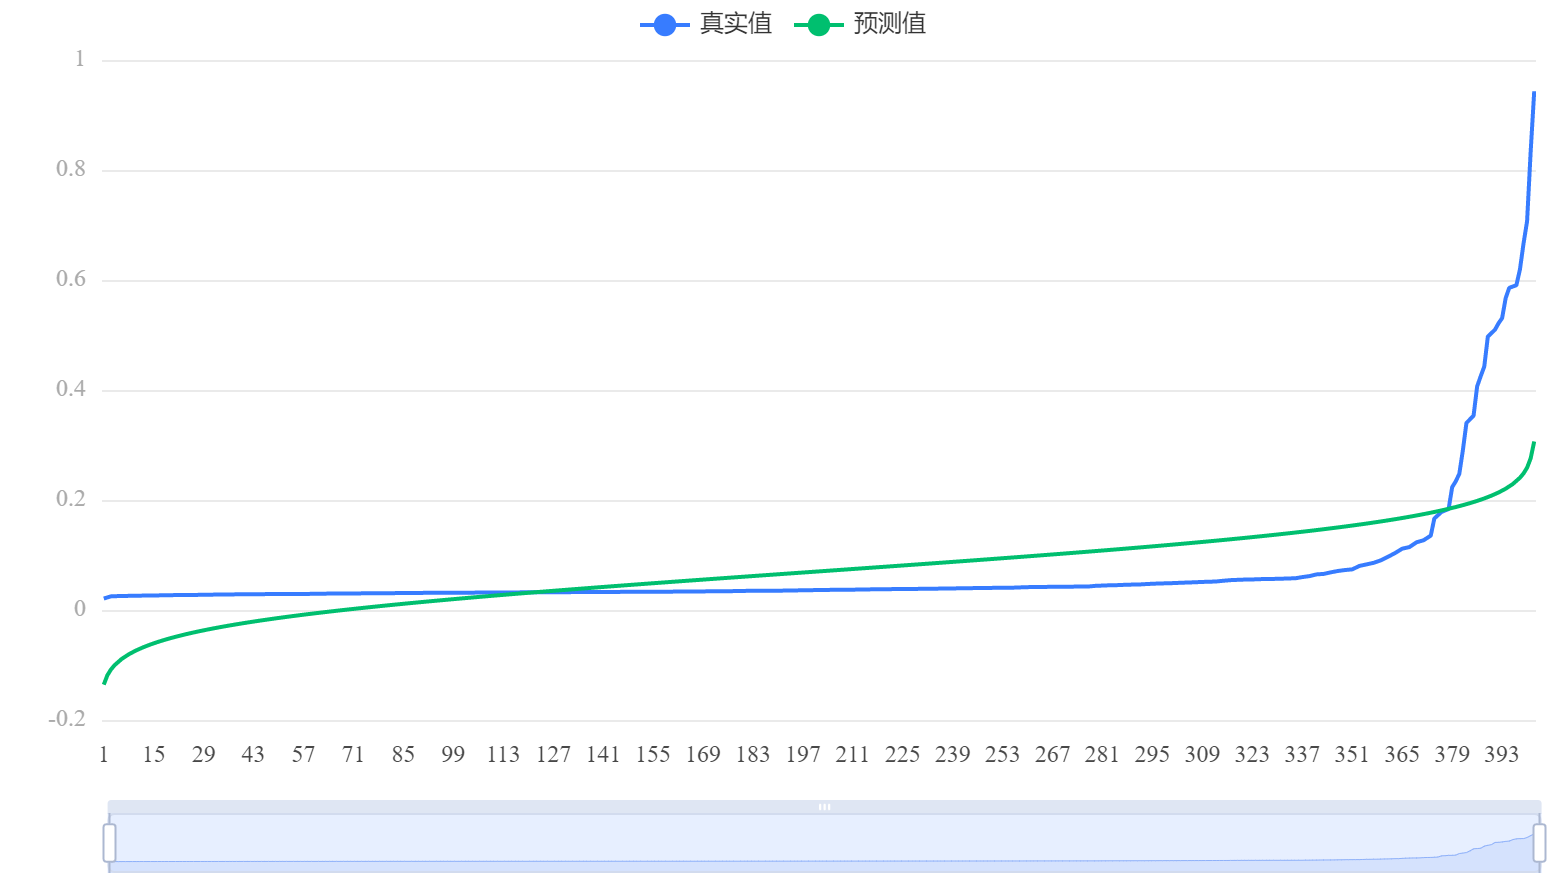
\includegraphics[width=0.45\textwidth]{img/fit.png} % 图片相对位置 
	\caption{拟合效果图} % 图片标题 
	\label{fig:figure 1} % 图片标签
\end{figure}

最后,我们得到分档排序临界值表格,尤其是Probit临界值对应的RSR临界值(拟合值)


我们根据综合主成分分析评价法和秩和比综合评价法分别得到供货商的评分PCA得分与RSR拟合值,我们将他们进行min-max处理,去除两个评分的量纲,将两个评价指标求和得到的综合得分作为最终的评价指标,取评分最高的Top50为最终选取的供应商。
\begin{center}
	\begin{longtable}{|c|c|c|c|c|c|c|}
		\caption{第二问预测结果}
		\label{tab:dasfa}                                                                              \\
		\hline
		供货商 & Probit      & RSR拟合值   & PCA得分     & PCA(标准化) & RSR拟合(标准化) & 综合评分值  \\ \hline
		228    & 8.228645179 & 0.306420133 & 2.782049173 & 1           & 1               & 2           \\ \hline
		360    & 7.808640011 & 0.275660741 & 2.601285883 & 0.950070052 & 0.930431451     & 1.880501503 \\ \hline
		274    & 7.243328763 & 0.23425975  & 2.3525052   & 0.881352524 & 0.836794786     & 1.718147309 \\ \hline
		328    & 7.110377294 & 0.224522951 & 2.333973533 & 0.876233757 & 0.814773057     & 1.691006814 \\ \hline
		339    & 7.172065188 & 0.229040709 & 2.278486776 & 0.860907354 & 0.824990875     & 1.68589823  \\ \hline
		267    & 6.921042354 & 0.210656865 & 2.278209629 & 0.860830802 & 0.783412116     & 1.644242918 \\ \hline
		130    & 7.006751594 & 0.216933845 & 2.126081771 & 0.818810455 & 0.797608768     & 1.616419224 \\ \hline
		107    & 7.577553464 & 0.258736946 & 1.713112255 & 0.704741131 & 0.892154886     & 1.596896017 \\ \hline
		305    & 6.847486818 & 0.20526997  & 2.120079287 & 0.817152466 & 0.77122857      & 1.588381035 \\ \hline
		193    & 6.782750875 & 0.200528985 & 2.129456061 & 0.819742493 & 0.760505879     & 1.580248372 \\ \hline
		281    & 7.055808328 & 0.220526552 & 1.905487341 & 0.757878458 & 0.805734397     & 1.563612855 \\ \hline
		246    & 6.623523182 & 0.188867826 & 1.864908952 & 0.746670005 & 0.734131823     & 1.480801828 \\ \hline
		351    & 6.753000099 & 0.198350165 & 1.783104178 & 0.724074111 & 0.75557804      & 1.47965215  \\ \hline
		139    & 7.434184791 & 0.248237234 & 1.283004136 & 0.585937828 & 0.868407676     & 1.454345504 \\ \hline
		355    & 6.814168805 & 0.202829901 & 1.603297148 & 0.674408299 & 0.765709863     & 1.440118162 \\ \hline
		150    & 7.328218628 & 0.240476723 & 1.257439062 & 0.578876312 & 0.85085572      & 1.429732032 \\ \hline
		30     & 6.557284368 & 0.184016778 & 1.704744368 & 0.702429776 & 0.723160203     & 1.425589979 \\ \hline
		307    & 6.962096557 & 0.2136635   & 1.380909307 & 0.61298093  & 0.790212225     & 1.403193155 \\ \hline
		329    & 6.882991702 & 0.207870197 & 1.286324272 & 0.586854907 & 0.777109506     & 1.363964413 \\ \hline
		293    & 6.298749674 & 0.165082796 & 1.584520457 & 0.669221852 & 0.680337196     & 1.349559048 \\ \hline
		364    & 6.478389768 & 0.178238873 & 1.440791839 & 0.629521521 & 0.710092309     & 1.33961383  \\ \hline
		142    & 6.724724606 & 0.196279388 & 1.284431535 & 0.5863321   & 0.750894561     & 1.337226661 \\ \hline
		265    & 6.216273909 & 0.159042622 & 1.48804126  & 0.642572628 & 0.666676128     & 1.309248756 \\ \hline
		345    & 6.328298237 & 0.167246807 & 1.313626842 & 0.594396349 & 0.685231542     & 1.279627891 \\ \hline
		39     & 6.460041725 & 0.17689514  & 1.18975455  & 0.560180679 & 0.707053187     & 1.267233866 \\ \hline
		283    & 6.536653804 & 0.182505883 & 1.081315281 & 0.530227877 & 0.71974301      & 1.249970887 \\ \hline
		366    & 6.391152774 & 0.171850006 & 1.086761145 & 0.531732119 & 0.695642602     & 1.227374721 \\ \hline
		122    & 6.165587919 & 0.155330596 & 1.162793881 & 0.552733676 & 0.658280635     & 1.211014311 \\ \hline
		217    & 6.242830371 & 0.160987505 & 1.108545615 & 0.537749366 & 0.671074872     & 1.208824238 \\ \hline
		363    & 6.42475216  & 0.174310682 & 0.967951043 & 0.498914713 & 0.701207916     & 1.200122628 \\ \hline
		243    & 6.256443485 & 0.161984471 & 1.051499232 & 0.521992168 & 0.673329711     & 1.195321879 \\ \hline
		79     & 6.284391587 & 0.164031271 & 1.006025901 & 0.509431647 & 0.677958961     & 1.187390608 \\ \hline
		66     & 6.061292014 & 0.147692408 & 1.050982553 & 0.521849452 & 0.641005337     & 1.16285479  \\ \hline
		138    & 6.671984578 & 0.192416933 & 0.656463001 & 0.412876327 & 0.742158842     & 1.15503517  \\ \hline
		188    & 6.129453754 & 0.152684284 & 0.972738958 & 0.500237218 & 0.652295468     & 1.152532686 \\ \hline
		212    & 6.05040415  & 0.146895027 & 0.954365241 & 0.495162079 & 0.6392019       & 1.134363979 \\ \hline
		350    & 5.810051726 & 0.129292638 & 1.084013747 & 0.53097324  & 0.599390558     & 1.130363798 \\ \hline
		75     & 6.072307165 & 0.14849911  & 0.85290527  & 0.46713708  & 0.642829856     & 1.109966936 \\ \hline
		396    & 5.759152739 & 0.125565012 & 1.029222365 & 0.515838912 & 0.590959782     & 1.106798694 \\ \hline
		4      & 6.028993803 & 0.145327024 & 0.866036047 & 0.470764028 & 0.635655546     & 1.106419574 \\ \hline
		394    & 6.600657784 & 0.187193262 & 0.488672451 & 0.366529674 & 0.73034446      & 1.096874135 \\ \hline
		179    & 5.734430232 & 0.123754441 & 0.981421551 & 0.5026355   & 0.586864812     & 1.089500312 \\ \hline
		200    & 6.697764393 & 0.194304937 & 0.40293102  & 0.342846408 & 0.746428943     & 1.089275351 \\ \hline
		347    & 6.647270359 & 0.190606969 & 0.388700859 & 0.338915791 & 0.738065245     & 1.076981036 \\ \hline
		54     & 6.374926512 & 0.170661664 & 0.537650657 & 0.380058302 & 0.692954928     & 1.07301323  \\ \hline
		45     & 5.987529589 & 0.142290361 & 0.759295529 & 0.44128045  & 0.628787522     & 1.070067972 \\ \hline
		6      & 6.153375681 & 0.154436224 & 0.627358189 & 0.404837074 & 0.656257833     & 1.061094907 \\ \hline
		365    & 5.726288885 & 0.123158204 & 0.873465466 & 0.472816162 & 0.585516302     & 1.058332464 \\ \hline
		97     & 6.039639404 & 0.146106663 & 0.681039986 & 0.419664916 & 0.637418856     & 1.057083772 \\ \hline
	\end{longtable}
\end{center}




\section{问题二的求解}
题目要求“参考问题 1”, 确定至少选择多少家供应商供应原材料才可能满足生产 的需求,。因此, 本文首先将供应商压缩为排名前 50 的 供应蔏, 继而针对这 50 家供应商, 建立 0-1 整数规划模型, 以满足生产需要的最少的 供应蔏数目为目标函数, 从而求解出选用哪几家供应商供应原材料, 并且这些供应商 的总数为多少。
\subsection{目标函数的构建}
为尽 可能选择少的供应商以满足生产的需要,本文从402家供应商中选出供货能力排名前50家供应商作为研究对象。所以,本文构建的目标函数为:

\begin{equation}
	\sum_{i=1}^{50}x_{ij}
\end{equation}

其中$x_{ij}$代表第i个供应商在第j周是否向该企业供货。若$x_{ij}$为1则代表供货,反之则代表没有供货。

\subsubsection{约束条件的构建}
\textbf{1.稳定供货能力}

为了求解满足企业生产需要的最少的供应商数量,本文当中假设每个供应商的供货量
达到自己的最大供货水平。但是从实际情况来看,对于一家供应商来说,
24周每周向企业提供的供应量不可能都是历史最大供货量,供货量也可能有起伏。
因此稳定的供货能力不能简单的视为最大的供货量,实际中稳定供货能力应小于或等于历史最大供货量。
定义供货系数为\textbf{B},\textbf{B}$\in\left ( 0, 1\right )$,使得:
\begin{equation}
	\mathbf{\textbf{\mbox{稳定的供货能力}}S_{ij} =B\cdot\textbf{\mbox{最大供货能力}}}
\end{equation}

\textbf{2.供给需求关系}

由于在第\textbf{j}周所有供货商的供货经过转运到达企业后应满足企业本周的生产需要
和库存需要,因此存在供给需求的等式关系,即该生产企业在第\textbf{j}周实际的原材料接
收量与第\textbf{j-1}周企业仓库中剩余的原材料库存量之和必须大于等于企业本周的产能所需
原材料量和两周生产需求的原材料库存量。为了便于计算,我们将等式两边的原材料
接收量与原材料库存量均转化为对应的企业产能,则供给需求关系式如下:
\begin{equation}
	\mathbf{\sum_{i=1}^{50} x_{ij}S_{ij}(1-L_{ij})f_{type}(i)+R_{j-1}=P+S_{2w}}
\end{equation}

其中,$\mathbf{f_{type}(i)}$为对原材料加工的转换函数,是计算将不同种类的
原材料转换成成品的函数。$\mathbf{S_{ij}}$表示第i个供货商在第j周给该企业的
供应量;$\mathbf{L_{ij}}$表示第i个供货商在第j周给该企业的供货过程中的损耗率;
$\mathbf{R_{j}}$表示在第j周后剩余库存转换为相应产能的产量,$\mathbf{P}$
表示企业的每周产能,$\mathbf{S_{2w}}$表示满足企业两周用量的原材料库存数量。

\textbf{3.损耗率}
在考虑第i个供货商在第j周发出的供货量在转运过程中的损耗率$\mathbf{L_{ij}}$时,
由于无法确定转运公司的选择,所以采用附件二中关于转运商240周的损耗率的平均值为损耗率,
统计出以24周为周期每周的平均损耗率,计算公式如下:
\begin{equation}
	\mathbf{L_{ij} =\bar{L} =\frac{\sum_{i=1}^{8}L_{jk} }{8}}
\end{equation}


这种情况下第i个供货和第l个在第j周的损耗率相同,则:
\begin{equation}
	\mathbf{L_{ij} =L_{lj} =\frac{\sum_{i=1}^{8}L_{jk} }{8}}
\end{equation}

\textbf{4.库存转换为产能}

根据题意,该企业要尽可能保持不少于两周生产需求的原材料库存量,因此,有
关系式如下:
\begin{equation}
	\mathbf{S_{2w}=2P}
\end{equation}

其中\textbf{P}为库存,$\mathbf{S_{2w}}$为产能。

\textbf{5.库存剩余量的计算迭代公式}

第j周的原材料库存剩余量$\mathbf{R_{j}}$,应等于第j周的原材料接收量与第j-1周的原
材料库存剩余量之和再减去第j周的产能所耗的原材料。本文将等式两边的原材料接收量
与原材料库存剩余量均转化为相应的产能,所以库存剩余量的迭代关系式如下:
\begin{equation}
	\mathbf{\begin{cases}
		R_{j}=\sum_{i=1}^{50}x_{ij}S_{ij}(1-L_{ij})f_{type}(i)+R_{j-1}-P  \\
		R_{j-1}=\sum_{i=1}^{50}x_{i(j-1)}S_{i(j-1)}(1-L_{i(j-1)})f_{type}(i)+R_{j-2}-P\\
		\cdot  \\
		\cdot  \\
		R_{1}=\sum_{i=1}^{50}x_{i1}S_{i1}(1-L_{i1})f_{type}(i)+R_{0}-P
		\end{cases}}
\end{equation}

\textbf{6.初始库存量}

在知道库存剩余量的迭代关系后,确定初始的库存剩余量$\mathbf{R_{0}}$至关重要。
考虑到企业依旧持有库存,所以在上一个为期24周的生产结束时企业不会将仓库中所
有的库存量全部生产用尽,因此不能简单的认为$\mathbf{R_{0}=0}$。

\begin{figure}[H]\centering
	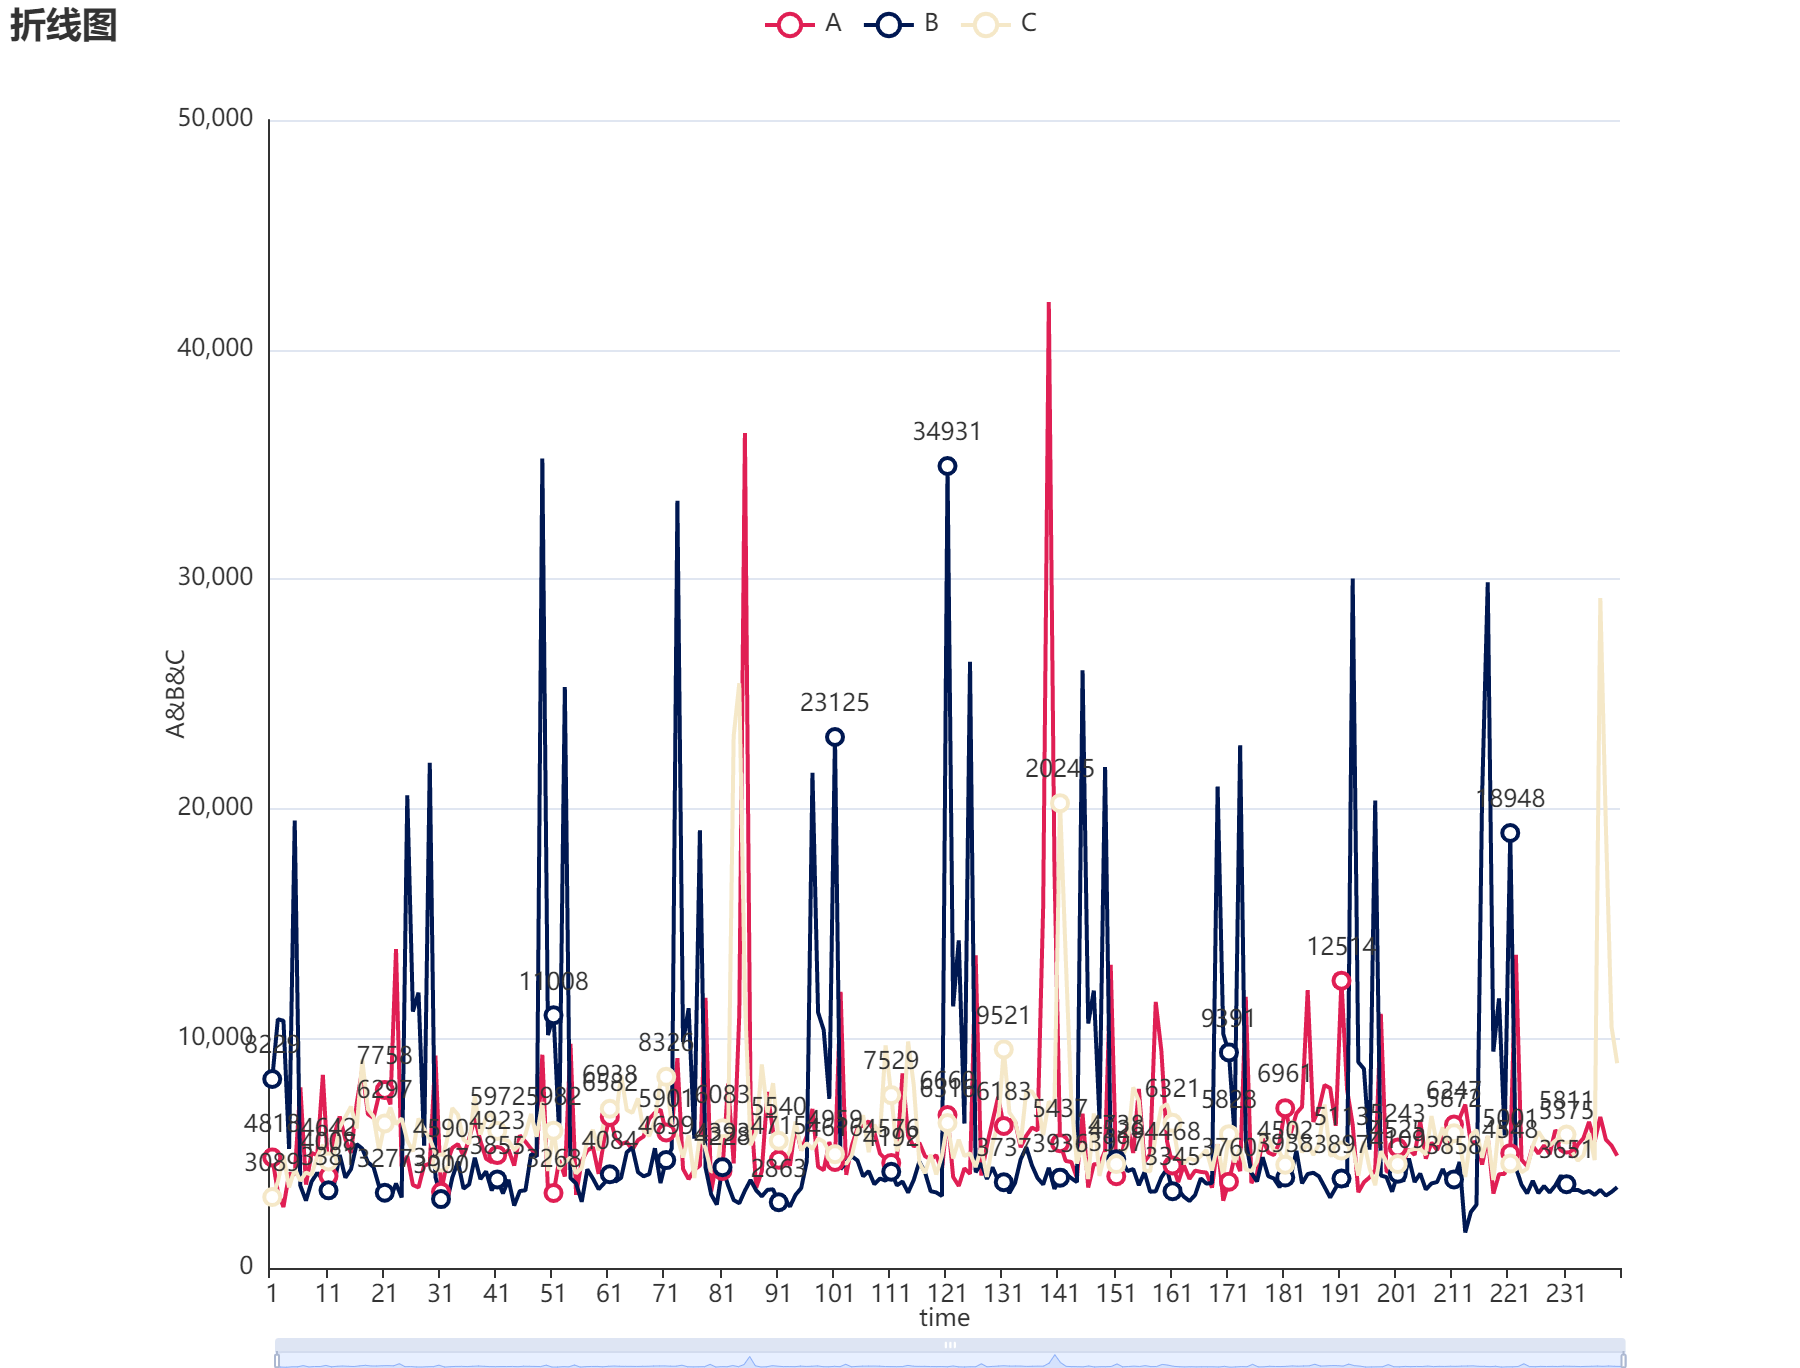
\includegraphics[width=1.2\textwidth,height=0.6\textwidth]{img/折线图 (1).png} % 图片相对位置 
	\caption{初始库存量} % 图片标题 
	\label{fig:figure 2} % 图片标签
\end{figure}

根据上图的订货量曲线不难发现订货量大致呈现随周期变化的规律,且周期长度
为24周。所以在以24周为周期的订购计划的开始,初始库存剩余量大致可用以往周
期的初始库存剩余量来计算.因此不妨设$\mathbf{R_{0}=S_{2w}}$。

\subsection{基于0-1整数规划的最少供应商模型}
在满足企业的生产需求的情况下,尽可能用最少的供应商向该企业提供生产的原
材料,结合已知条件和假设,基于0-1整数规划的最少供应商模型确立为:
\begin{equation}
	\sum_{i=1}^{50}x_{ij}
\end{equation}\par
~~~~~~~~~~~~~~~~~~~~~~~~~~~s.t$\mathbf{\begin{cases}
	\sum_{i=1}^{50} x_{ij}S_{ij}(1-L_{ij})f_{type}(i)+R_{j-1}=P+S_{2w}  \\
	R_{j-1}=\sum_{i=1}^{50}x_{i(j-1)}S_{i(j-1)}(1-L_{i(j-1)})f_{type}(i)+R_{j-2}-P\\
	L_{ij}=\bar{L}  \\
	S_{ij}=B\cdot \makebox{最大供货能力}  \\
	R_{0}=S_{2w}   \\
	S_{2w}=2P
	\end{cases}}$

	需要注意:由于迭代,该0-1整数规划模型对于每个j(即周)都是一个全新的规划。
\subsection{问题二最少供应商模型求解}
在满足生产需求的情况下的得到最少的供应商数为24个,结果如下:

\begin{center}
	\begin{tabular}{||c c c c||}
		\hline
		S229 & S308 & S356 & S247      \\ [0.5ex]
		\hline
		S361 & S282 & S268 & S284      \\
		\hline
		S151 & S340 & S306 & S055      \\
		\hline
		S108 & S275 & S194 & S201      \\
		\hline
		S330 & S329 & S143 & S003      \\
		\hline
		S229 & S131 & S352 & S037      \\
		\hline
	\end{tabular}
\end{center}

\subsection{基于线性规划的最经济订购方案模型的建立}
为了制定未来24周每周“最经济"的原材料订购方案,本文针对上述模型求解出的
24家原材料供应商,建立线性规划模型,在必须满足企业的生产需求的约束条件下,
以24周该生产企业需要给原材料供应商的采购费用和给物流公司(即转运商)的运
输费用以及在仓库储存费用之和达到最小作为目标函数,从而确定出24家原材料供
应商每周接到的订货量(总共24周)。
\subsubsection{目标函数的构建}
由于制定订购方案需要明确该生产企业需要订购的原材料供应商以及向这些供应
商每周(总共24周)订购的订货量,因此我们选择以第i家供应商在第j周接到的订
货量为自变量,即$\mathbf{O_{ij}}$。根据题目要求,本文此处的供应商已经
确定为上述0-1整数规划模型所求解得到的24家供应商,因此i=1,2...24, j=1,2...24. 
以240周内所有供应商提供的总供货量在采购和运输以及储存该三方面花费的成本最小构造目标
函数,表达式如下:
\begin{equation}
	\mathbf{min\sum_{i=1}^{24} \sum_{j=1}^{24}O_{ij}(1-r_{oS_{ij}})(r_{i}p+c)}
\end{equation}
\subsubsection{约束条件的构建}
由于订购方案是为了满足企业的正常生产需求,因此本文此处的约束条件与基于
0-1整数规划的最少供应商模型相同,只是变量的表示发生了变化,因此此处不再多
余赘述约束条件的构建。
\subsubsection{基于线性规划的最经济订购方案模型}
为了制定未来24周每周最经济的订购方案,即要求订购的原材料总量在采购、运
输及储存三方面的成本花费为最小,在制定方案的同时也需要保证该订购方案满足企
业的生产需求,结合已知条件和假设,该规划模型需要满足以下约束:

1.该生产企业对一周的原材料接收量和上一周剩余的原材料库存量的总和不少于
满足两周生产需要的原材料库存量与一周的产能需要的原材料的总和。

2.一周的原材料库存量是来源于该周的原材料接收量与上一周剩余的原材料库存
量的总和中除去该周的产能需要的原材料量后剩余的数量。

3.该生产企业第一周的库存量为两倍的产能所需原材料。

4.该企业尽可能保持不少于满足两周生产需求的原材料库存量。

5.为了计算方便,本文将原材料的接收量和库存量转换为相应的等量产能。

因此,基于线性规划的最经济订购方案模型确立为:
\begin{equation}
	\mathbf{min\sum_{i=1}^{24} \sum_{j=1}^{24}O_{ij}(1-r_{oS_{ij}})(r_{i}r_{1}+r_{2})}
\end{equation}\par
~~~~~~~~~~~~~~~~~~~~~~~~~~~s.t$\mathbf{\begin{cases}
	\sum_{i=1}^{24}x_{ij}O_{ij}(1-r_{OS_{ij}}(1-L_{ij})f_{type}(i)+R_{i-1}=P+S_{2w}  \\
	R_{j-1}=\sum_{i=1}^{50}x_{i(j-1)}O_{i(j-1)}(1-r_{OS_{ij}}(1-L_{i(j-1)})f_{type}(i)+R_{j-2}-P_{i} \\
	L_{ij}=\bar{L}  \\
	r_{OS_{ij}}=\bar{r_{OS_{ij}}}  \\
	R_{0}=S_{2w}   \\
	S_{2w}=2P
	\end{cases}}$

其中,$\mathbf{r_{OS_{ij}}}$表示以240周为时间总长,24周为一个单位时间长度得到的第i家供应
商在第j周的平均订购偏差率,$\mathbf{r_{i}}$是第i个供应商供应的原材料的采购单价相对C类原
材料采购单价的比值,其可能取值为$\mathbf{\left \{1.2,1.1,1  \right \} }$,$\mathbf{P}$表示C类原材料的采购单价,$\mathbf{C}$
表示原材料运输和储存的单位费用。


\subsection{基于线性规划的最经济订购方案模型的求解}
\textbf{方案实施效果分析:}

根据本文模型建立的原理,每周8家转运商总转运量应大致
等于该周向24家供应商订货总数,输出结果显示求解结果与预期吻合。此外,可
知24周平均每立方米原材料需单位成本如下,可见订购方案较为经济。
\begin{center}
	\begin{tabular}{||c c c c c c c c c c c c||}
		\hline
		1 & 2 & 3 & 4 & 5 & 6 & 7 & 8 & 9 & 10 & 11 & 12     \\ [0.5ex]
		\hline
		1.60 & 1.61 & 1.57 & 1.57 & 1.62 & 1.56 & 1.57 & 1.58 & 1.58 & 1.62 & 1.52 & 1.55      \\
		\hline
		13 & 14 & 15 & 16 & 17 & 18 & 19 & 20 & 21 & 22 & 23 & 24      \\
		\hline
		1.65 & 1.65 & 1.57 & 1.57 & 1.65 & 1.57  & 1.57 & 1.65 & 1.57 & 1.57 & 1.65 & 1.60     \\
		\hline
	\end{tabular}
\end{center}

\subsection{基于线性规划的最少转运损耗方案模型的建立}
根据上述基于线性规划的最经济订购方案模型,可以得到24家供应商每周接到
的订购量,据此来制定每周内每家供应商的供货量分配给哪一家/几家转运商来运输,
并以每家转运商的运输能力为6000立方米/周作为约束条件之一,建立线性规划模型,
以8家转运商在24周的转运过程中的总损耗量最少为目标函数,从而确定出每周每
家转运商转运哪一家/几家供货商的供货量。

由于过去的转运损耗不会影响本周的转运损耗,所以要使转
运损耗最小只需要使每周的转运损耗都最小,为了简便计算可以一周为单位考虑。假
设第j(j=1,2....24)周第i(i=1, 2....24)家供货商由第k(k=1, 2...8)家转运公
司转运的原材料量为$\mathbf{T_{ik}}$,该转运公司的转运损耗率为$\mathbf{L_{k}}$,
则第j周所有货物的总损耗
为$\mathbf{\sum_{i}^{24}\sum_{k=1}^{8}T_{ik}L_{k}}$,所以为了使得转运损耗最小,
有目标函数:
\begin{equation}
	\mathbf{\min \sum_{i=1}^{24} \sum_{k=1}^{8} T_{i k} L_{k}, \text { for } j=1,2, \ldots, 24}
\end{equation}\par
\subsubsection{约束条件的建立}
\textbf{1.转运损失率}

由于同一个转运公司不同时间转运的损耗率不同, 且由上文可知, 整个订购运送过程
具有周期性, 近 5 年共有 10 个周期, 周期为 24 周, 故转运公司  k  在第  j  周
的转 运损失率可以用以往 10 个周期中第  j  周转运损失率的均值$\mathbf{\bar{L}(k, j)}$  
表示, 计算关系式 如下:
\begin{equation}
	\mathbf{L_{k}=\bar{L}(k, j)}
\end{equation}

\textbf{2.承接量}

根据题意每家转运商的运轵能力为 6000 立方米/周, 所以第  k  家转运公司在 24 周内
给第i家企业转运原材料的总量不大于 6000 (单位: 立方米), 不等式如下:
\begin{equation}
	\mathbf{\sum_{i=1}^{24} T_{i k} \leqslant 6000, \text { for } k=1,2, \ldots, 8}
\end{equation}

\textbf{3.供货量}

若第i家供货商由第k家转运公司转运的原材科量为$\mathbf{T_{ik}}$, 则该供货商由各个转运商
转运的原材料量的总和应该为该供货商的总供货量, 即:
\begin{equation}
	\mathbf{\sum_{k=1}^{8} T_{i k}=S_{i}, \text { for } i=1,2, \ldots, 24}
\end{equation}

其中,$\mathbf{S_{i}}$为第i家供货商在第j天的给定的总供货量。
\subsubsection{基于线性规划的最经济转运方案模型}
基于线性规划的最经济转运方案模型确立为:
\begin{equation}
	\mathbf{\begin{array}{c}
	\min \sum_{i=1}^{24} \sum_{k=1}^{8} T_{i k} L_{k} \\
	\text { s.t. }\left\{\begin{array}{l}
	L_{k}=\bar{L}(k, j) \\
	\sum_{i=1}^{24} T_{i k} \leqslant 6000, \text { for } k=1,2, \ldots, 8 \\
	\sum_{k=1}^{8} T_{i k}=S_{i}, \text { for } i=1,2, \ldots, 24
	\end{array}\right.
	\end{array}}
\end{equation}

该线性规划模型只针对求解一周的转运方案, 为了获得24周的转运方案, 则需要重复使用该模型, 
其中$\mathbf{T_{ik},L_{k}, S_{i}}$都会随着周数的改变而改变。但因为两个约束条件分别是
关于24周每周的约束条件和8家转运商每家的约束条件,所以该模型的可解性是一定被保证的。

\subsection{基于线性规划的最少损耗转运方案模型的求解}
\textbf{方案实施效果分析:}

24周平均每周转运损耗率如下,可见转运方案转运效率良好:
\begin{center}
	\begin{tabular}{||c c c c c c ||}
		\hline 
		1 & 2 & 3 & 4 & 5 & 6   \\
		\hline 
		0.1397 & 0.2122 & 0.1717 & 0.1859 & 0.2003 & 0.2567 \\
		\hline 
		7 & 8 & 9 & 10 & 11 & 12 \\
		\hline
		0.1189 & 0.0280 & 0.1960 & 0.2439 & 0.1233 & 0.2115 \\
		\hline 
		13 & 14 & 15 & 16 & 17 & 18 \\
		\hline 
		0.2936 & 0.3483 & 0.3442 & 0.1412 & 0.4659 & 0.4881 \\
		\hline 
		19 & 20 & 21 & 22 & 23 & 24 \\
		\hline 
		0.1621 & 0.1621 & 0.1621 & 0.1621 & 0.1621 & 0.1621 \\
		\hline
	\end{tabular}
\end{center}

\section{问题三的求解}


%引用
\clearpage
\bibliographystyle{plain}
\bibliography{ref}%ref指向自己创建的ref.bib
% IoU\cite{zheng2020distance}
\clearpage

\section{附录}
\subsection{代码}
\subsubsection{第一问代码}
\lstset{language=python}
\begin{lstlisting}
	import numpy as np
	import pandas as pd
	from copy import deepcopy
	
	# 数据读取
	data1 = np.array(pd.read_excel('./excel/附件1近5年402家供应商的相关数据.xlsx', sheet_name=0).fillna(0))
	data2 = np.array(pd.read_excel('./excel/附件1近5年402家供应商的相关数据.xlsx', sheet_name=4).fillna(0))
	
	data_order = data1[:, 2:]
	data_supply = data2[:, 2:]
	data_supplier = data1[:, 0:2]
	
	#  计算各供应商订货量/供货量能够生产的产品数
	data_order2 = np.zeros(data_order.shape)
	for i in range(data_order.shape[0]):
		if data_supplier[i, 1] == 'A':
			data_order2[i] = data_order[i] * (1 / 0.6)
		elif data_supplier[i, 1] == 'B':
			data_order2[i] = data_order[i] * (1 / 0.66)
		else:
			data_order2[i] = data_order[i] * (1 / 0.72)
	# data_order2= data_order2.sum()  / 240
	
	data_supply2 = np.zeros(data_supply.shape)
	for i in range(data_supply.shape[0]):
		if data_supplier[i, 1] == 'A':
			data_supply2[i] = data_supply[i] * (1 / 0.6)
		elif data_supplier[i, 1] == 'B':
			data_supply2[i] = data_supply[i] * (1 / 0.66)
		else:
			data_supply2[i] = data_supply[i] * (1 / 0.72)
	
	# 供货数量
	supply_num = data_supply2.sum(axis=1)
	# 供货稳定指数 1/(供货量变异系数+1)
	supply_stability = np.array(
		[np.std(data_supply2[k][data_order2[k] != 0]) / np.mean(data_supply2[k][data_order2[k] != 0])
		 for k in range(402)])
	supply_stability2 = 1 / (supply_stability + 1)
	# 供货偏移指数 1/(供货量与订货量差的平方平均数+1)
	diff = data_supply2 - data_order2
	supply_shift = []
	for k in range(402):
		shift_i = np.mean(np.square(diff[k][data_order2[k] != 0] / data_order2[k][data_order2[k] != 0]))
		supply_shift.append(shift_i)
	supply_shift = np.array(supply_shift)
	supply_shift2 = 1 / (supply_shift + 1)
	# 订货数量
	order_num = data_order2.sum(axis=1)
	# 订货稳定指数  1/(订货量的变异系数+1)
	order_stability = np.array(
		[np.std(data_order2[k][data_order2[k] != 0]) / np.mean(data_order2[k][data_order2[k] != 0])
		 for k in range(402)])
	order_stability2 = 1 / (order_stability + 1)
	# 供应商占用率 1-闲置率
	vacancy_rate = (data_order == 0).sum(axis=1) / 240
	vacancy_rate2 = 1 - vacancy_rate
	# 供应商守约率 1-违约
	default_rate = ((data_order > 0) & (data_supply == 0)).sum(axis=1) / (data_order != 0).sum(axis=1)
	default_rate2 = 1 - default_rate
	# 重要订单接收频次
	important_freq = np.zeros(402)
	for i in range(data_order2.shape[1]):
		index = np.argsort(data_order2[:, i])[::-1][0:20]
		important_freq[index] += 1
	# 供应商细分市场份额
	all = np.zeros(402)
	for i in range(len(all)):
		if data_supplier[i, 1] == 'A':
			all[i] = np.sum(data_supply2[data_supplier[:, 1] == "A", :])
		elif data_supplier[i, 1] == 'B':
			all[i] = np.sum(data_supply2[data_supplier[:, 1] == "B", :])
		else:
			all[i] = np.sum(data_supply2[data_supplier[:, 1] == "C", :])
	segmentation_market_share = data_supply2.sum(axis=1) / all
	
	# 整合各特征
	data_feature = np.vstack([supply_num, supply_stability2, supply_shift2, order_num, order_stability2, important_freq,
							  segmentation_market_share, vacancy_rate2, default_rate2]).T
	
	# 特征数据输出
	data_out = pd.DataFrame(data_feature)
	data_out.columns = ['供货数量', '供货稳定指数', '供货偏移指数', '订货数量', '订货稳定指数', '重要订单接受频次',
						'供应商细分市场份额', '供应商占用率', '供应商守约率']
	data_out.to_excel('第1问参数数值.xlsx')
	
	# 特征归一化处理
	from sklearn.preprocessing import MinMaxScaler
	
	feature_scaled = deepcopy(data_feature)
	feature_scaled[:, [0, 3, 5]] = MinMaxScaler().fit_transform(feature_scaled[:, [0, 3, 5]])
	
	# 主成分加权
	from sklearn.decomposition import PCA
	
	pca = PCA(svd_solver='full')
	feature_pca = pca.fit_transform(feature_scaled)
	variance = pca.explained_variance_ratio_.reshape(-1, 1)
	supplier_score = feature_pca @ variance
	components = pca.components_
	pd.DataFrame(supplier_score).to_excel('供应商得分.xlsx')  # 输出402家企业加权得分
	pd.DataFrame(np.hstack((variance, components))).to_excel('主成分.xlsx')  # 输出主成分的参数
	
	# 计算各企业最大供应量
	max_offer = data_supply2.max(axis=1).reshape(-1, 1)
	a = np.hstack((supplier_score, max_offer))
	a = a[np.argsort(a[:, 0])[::-1]]  # a从大到小排序
	m = np.array([a[:i, 1].sum() for i in range(50)])


		
\end{lstlisting}
\subsubsection{问题二代码}
\lstset{language=python}
\begin{lstlisting}
import pandas as pd
import numpy as np
from matplotlib import pyplot as plt
import seaborn as sns
import numpy as np 
import cvxpy as cp
from scipy import optimize as op 

pred_result = pd.read_csv('TSA_decided.csv')
pred_result['id'] = pred_result['Unnamed: 0']+1

pred_result.set_index('id',inplace=True)
pred_result.drop('Unnamed: 0',axis=1, inplace=True)
candidates = pd.read_csv('n_sup_decided.csv')
candidates['n_id'] = [int(x[1:]) for x in candidates['id'].values]
selected = candidates.loc[range(50)]

selected.supply_amount.values.sum()/5

avg_need_eqC = (2.82*10**4)*0.72
'每周生产需求(eqC):'+str((2.82*10**4)*0.72)

trans = pd.read_csv('trans.csv')
def replace0(x):
    if x == 0:
        return np.nan
    else:
        return x
    
notnull = 8*240 - trans.isnull().sum().sum()
avg_los = (trans.sum().values[1:].sum()/notnull)*0.01

'有运输时的平均货损率:'+str(avg_los)

selected_pred = pred_result.loc[selected['n_id'].values]

month_sup_50 = selected_pred.sum(axis=0)
need_array_eqC = np.array([avg_need_eqC for i in range(24)])
plt.figure(figsize=[30,4])
plt.xticks(range(1,25))


plt.bar(x=range(1,25), height=month_sup_50, label='month_sup_50', color='darkred')
plt.bar(x=range(1,25), height=need_array_eqC, label='need_array_eqC', color='darkgray',alpha=0.7)

plt.legend()
plt.title('50 Need & Supply Barplot')
plt.savefig('50 Need & Supply Barplot.jpg')

selected_pred.sort_index(inplace=True)
selected_pred.to_csv('for_matlab.csv')
selected_pred = selected_pred.T
for i in range(len(selected_pred)):
    if i<=22:
        selected_pred.iloc[i+1] = selected_pred.iloc[i+1] + selected_pred.iloc[i]


		c = np.array([1 for i in range(50)])

		a = np.array(selected_pred)
		
		b = np.array([avg_need_eqC*i for i in range(1,25)])
		
		x = cp.Variable(50,integer=True)
		
		obj = cp.Minimize(c*x)
		
		cons =[a*x>=b, x>=0, x<=1]
		
		prob =cp.Problem(obj, cons)
		
		prob.solve( solver='GLPK_MI', verbose=True)

		order_eqC = pd.read_csv('supply_eqC.csv')


order_eqC['id'] = [int(x[1:]) for x in order_eqC['供应商ID'].values]
selected_eqC = order_eqC.set_index('id').loc[opt_res1_df.id]


\end{lstlisting}
\end{document}
